\documentclass[tikz,border=4pt]{standalone}
\usepackage{amsmath}
\usepackage{xcolor}
\usepackage{xspace}
\usepackage{tikz}
\usetikzlibrary{arrows.meta,positioning,fit,backgrounds,shapes.geometric}

\definecolor{caraprimary}{RGB}{30,60,120}
\definecolor{caraaccent}{RGB}{200,80,60}
\newcommand{\effnet}{EfficientNet-B0\xspace}

\begin{document}
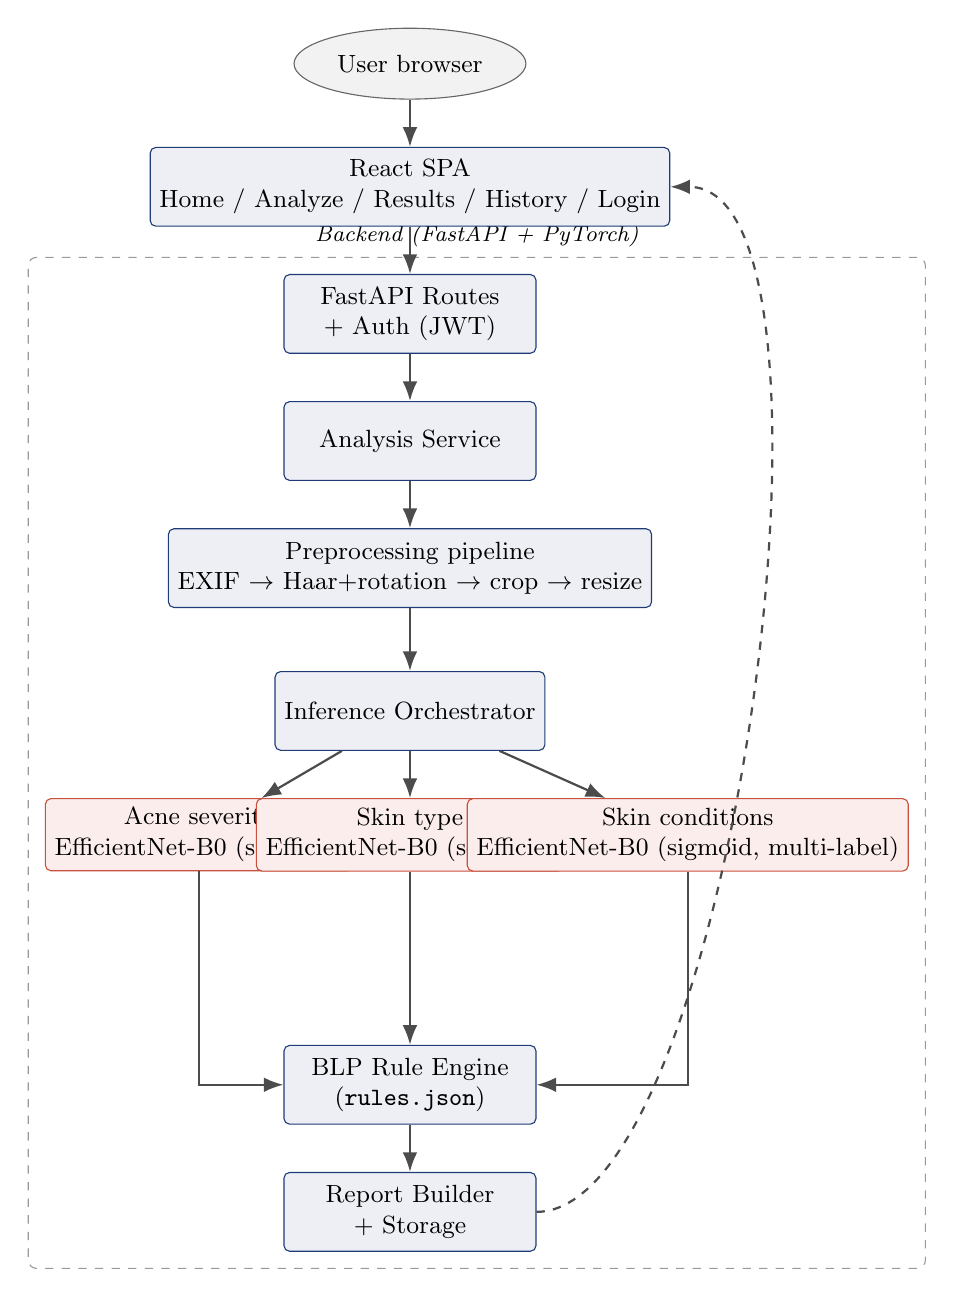
\begin{tikzpicture}[
    node distance=6mm and 10mm,
    every node/.style={font=\small},
    service/.style={rectangle, draw=caraprimary, fill=caraprimary!8,
        minimum height=1.0cm, minimum width=3.2cm, rounded corners=2pt,
        align=center},
    model/.style={rectangle, draw=caraaccent, fill=caraaccent!10,
        minimum height=0.9cm, minimum width=3.2cm, rounded corners=2pt,
        align=center},
    io/.style={ellipse, draw=black!60, fill=black!5, align=center,
        minimum height=0.9cm, minimum width=2.6cm},
    arrow/.style={-{Latex[length=2.5mm]}, thick, draw=black!70}]

    \node[io]                        (user)  {User browser};
    \node[service, below=of user]    (front) {React SPA\\Home / Analyze / Results / History / Login};
    \node[service, below=of front]   (api)   {FastAPI Routes\\+ Auth (JWT)};
    \node[service, below=of api]     (svc)   {Analysis Service};
    \node[service, below=of svc]     (pre)   {Preprocessing pipeline\\EXIF \(\to\) Haar+rotation \(\to\) crop \(\to\) resize};

    \node[service, below=8mm of pre] (orch)  {Inference Orchestrator};
    \node[model, below left=6mm and -10mm of orch] (m1) {Acne severity\\\effnet (softmax)};
    \node[model, below=6mm of orch]                (m2) {Skin type\\\effnet (softmax)};
    \node[model, below right=6mm and -10mm of orch](m3) {Skin conditions\\\effnet (sigmoid, multi-label)};

    \node[service, below=22mm of m2] (blp)  {BLP Rule Engine\\(\texttt{rules.json})};
    \node[service, below=of blp]     (rep)  {Report Builder\\+ Storage};

    \draw[arrow] (user)  -- (front);
    \draw[arrow] (front) -- (api);
    \draw[arrow] (api)   -- (svc);
    \draw[arrow] (svc)   -- (pre);
    \draw[arrow] (pre)   -- (orch);
    \draw[arrow] (orch)  -- (m1);
    \draw[arrow] (orch)  -- (m2);
    \draw[arrow] (orch)  -- (m3);
    \draw[arrow] (m1) |- (blp);
    \draw[arrow] (m2) -- (blp);
    \draw[arrow] (m3) |- (blp);
    \draw[arrow] (blp)   -- (rep);
    \draw[arrow, dashed] (rep.east) .. controls +(right:2.5cm) and +(right:2.5cm) .. (front.east);

    \begin{scope}[on background layer]
        \node[draw=black!40, dashed, rounded corners=3pt,
              fit=(api)(svc)(pre)(orch)(m1)(m2)(m3)(blp)(rep),
              inner sep=6pt, label={[font=\footnotesize\itshape]above:Backend (FastAPI + PyTorch)}] {};
    \end{scope}
\end{tikzpicture}
\end{document}
